%%%%%%%%%%%%%%%%%%%%%%%%%%%%%%%%%%%%%%%%%%%%%%%%%%%%%%%%%%%%%%%%%%%%%%%%%%%%%%
%
% Appendix file included in main project file using \input{}
%
% Assumes that LaTeX2e macros and packages defined in cg_comp.sty are
%   available
%
%%%%%%%%%%%%%%%%%%%%%%%%%%%%%%%%%%%%%%%%%%%%%%%%%%%%%%%%%%%%%%%%%%%%%%%%%%%%%%

 \section{Fretting Model\label{app:fret}}

As discussed in \sct{model}, we have neglected to include a contribution to the incremental change in the length of the fretted string caused by both the depth and the shape of the string under the finger~\cite{ref:byers1996cgi,ref:varieschi2010icf}. Here we include this concept in a simple way to determine the effect it could have on the frequency shift due to increased string tension. In \fig{fretting_schematic}, we adopt the schematic of the guitar shown in \fig{guitar_schematic}, but we allow a small, horizontal linear section of string with length $d$ to represent the action of the finger. In this case, the resonant length $L_n$ is unaffected, but the remaining string length becomes
 \begin{equation}
L^\prime_n = d + \sqrt{\left(X_0 + \Delta N - X_n - d\right)^2 + b^2} \approx X_0 - X_n + \Delta N + \frac{b^2}{2 \left(X_0 + \Delta N - X_n - d\right)}\, .
 \end{equation}
Roughly speaking, the act of fretting increases the effective value of $b^2$ in $L^\prime_n$ by a factor of $1 + d / (X_0 - X_n)$. We can use \eqn{q_n_def} to determine the increase in the relative displacement $Q_n$.

In \fig{fret_disp}, we plot $Q_n$ for the first three frets as a function of the distance parameter $d$. For this example, we have adopted the parameters of an Alhambra 8P guitar using normal tension strings. In the worst case, where $d = 1$~cm, $Q_1$ increases by almost $8.0 \times 10^{-6}$. For string 3 (G) in \tbl{ej45_props}, we see that $\kappa = 111$, and in \fig{fret_shift} we plot $\Delta \nu_n(d) - \Delta \nu_n(0)$ as a function of $d$ for that string. Despite this high value of $\kappa$ and the prediction in \fig{fret_shift} that the shift on the first fret could increase by as much as 0.8~cents, our measurements for $\Delta \nu_1$ using the Alhambra 8P guitar and normal tension strings is consistent with the theoretical values using $d = 0$ shown in \fig{shift_alhambra8p_ej45_factory}. Therefore, without a compelling reason to do so, we are reluctant to choose a value of $d$ greater than 0. It is true that we can press the string so hard that it touches the fret board, increasing the frequency shift by as much as 2 -- 3 cents, but this is likely the result of dragging the string over the fret and causing a local change in tension that is inconsistent with the boundary conditions used to derive \eqn{f_m_stiff}.

 \begin{figure}
  \centering
  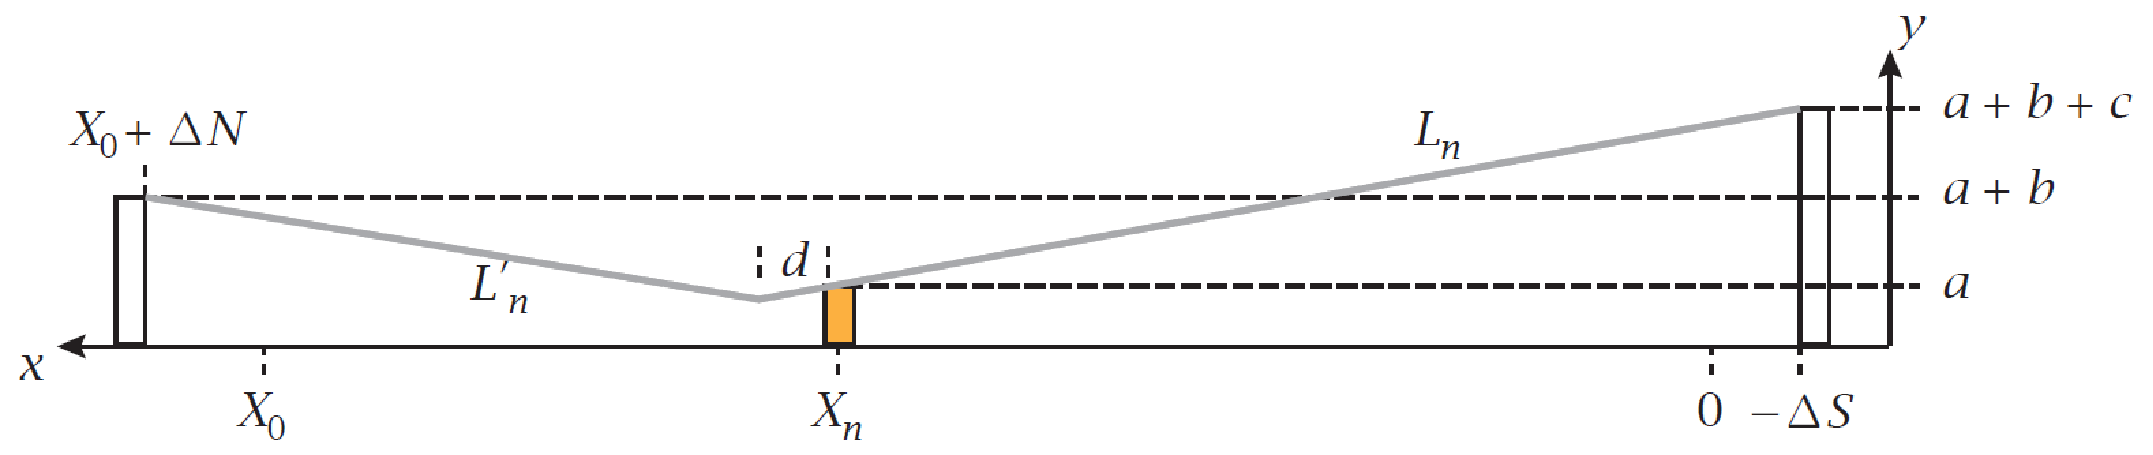
\includegraphics[width=6.0in]{figures/fretting_schematic}
  \caption{\label{fig:fretting_schematic} A recapitulation of \fig{guitar_schematic} with the addition of a horizontal linear distance $d$ at fret $n$ to represent the slight increase in the distance $L_n^\prime$ caused by a finger.}
 \end{figure}

 \begin{figure}
  \centering
  \begin{subfigure}[b]{0.8\textwidth}
   \centering
   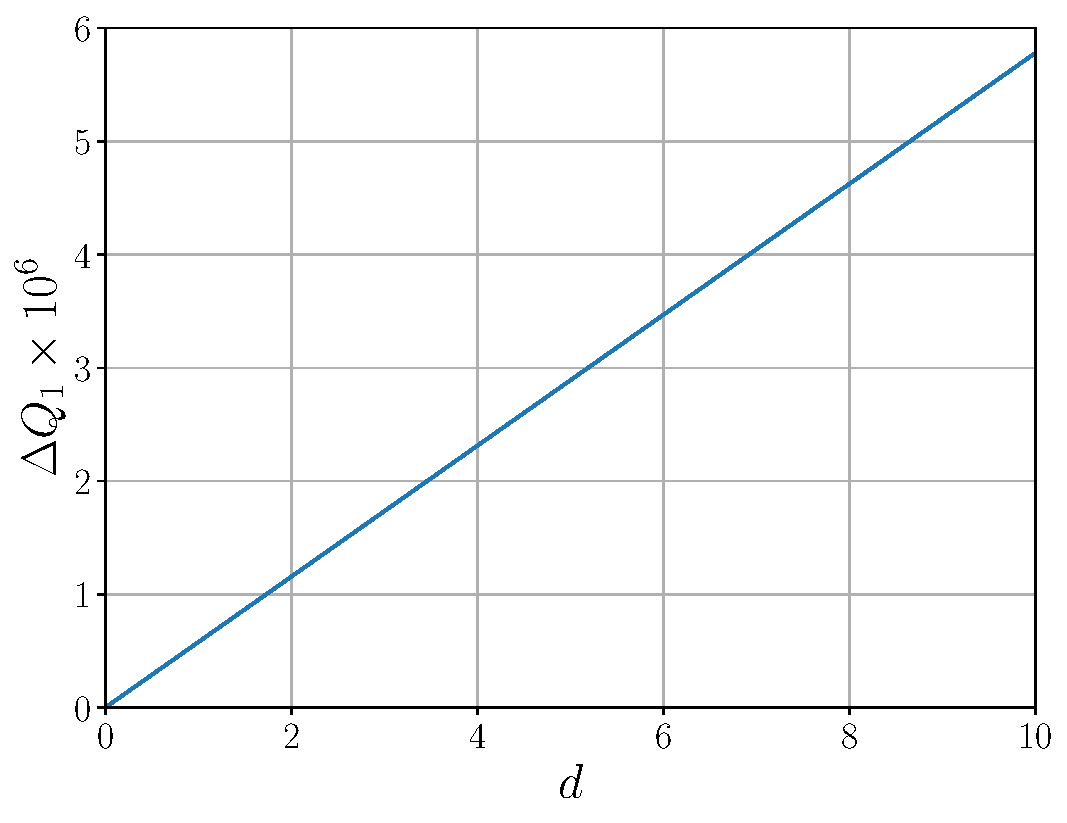
\includegraphics[width=5.0in]{figures/fret_disp}
   \caption{Relative displacement $Q_n$}
   \label{fig:fret_disp}
  \end{subfigure}
  \par\vspace{0.25in}
  \begin{subfigure}[b]{0.8\textwidth}
   \centering
   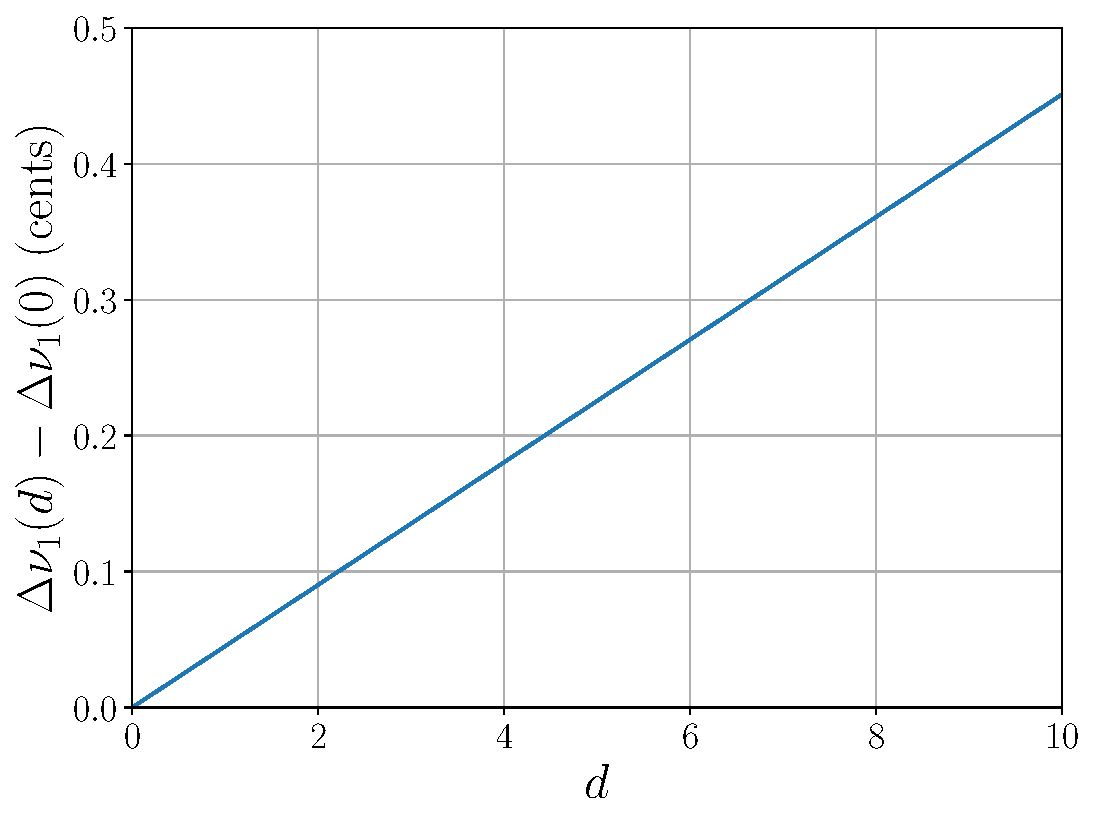
\includegraphics[width=5.0in]{figures/fret_shift}
   \caption{Additional frequency shift of string 3}
   \label{fig:fret_shift}
  \end{subfigure}
  \caption{\label{fig:fret_model} In (a), we plot the relative displacement $Q_n$ for the first three frets as a function of the fretting distance parameter $d$. Here the guitar has the same parameters as the Alhambra 8P, with normal tension strings. In (b), we show the additional frequency shift of the third string --- with $\kappa = 111$ --- as $d$ increases from 0. For $n > 3$, the additional shift is even smaller.}
 \end{figure}
